% !TeX encoding = UTF-8
% !TeX program = xelatex
% !TeX spellcheck = en_US

\documentclass[a4paper]{ltxdoc}
\usepackage{amsmath}
\usepackage[UTF8]{ctex}
\usepackage{unicode-math}
\usepackage{caption}
\usepackage{booktabs}
\usepackage{xcolor}
\usepackage{array}
\usepackage{listings}
\usepackage[perpage]{footmisc}
\usepackage{hypdoc}
\usepackage{geometry}
\usepackage{endnotes}
\usepackage{graphicx}
% \usepackage[multiple]{endnotes}
\usepackage{multicol}
\usepackage{blindtext}
\geometry{a4paper, scale=0.85}
\newenvironment{Figure}
  {\par\medskip\noindent\minipage{\linewidth}}
  {\endminipage\par\medskip}

\title{实验报告\\自由落体法测量重力加速度}
\author{少年班学院\\马天开 PB21000030(第三组)}
\date{\today}

\begin{document}
\begin{multicols}{2}
    \maketitle
    \section{实验背景}
    参考“实验报告:单摆法测量重力加速度”
    \section{实验目的}
    参考“实验报告:单摆法测量重力加速度”
    \section{实验器材}
    光电门$\times 2$、电磁铁控制器(可以控制磁性的有无)、小铁球、带刻度的支架、电子计时器

    光电门精度:$1\times 10^{-4} s$,支架上刻度的测量精度:$10^{-3}m$
    \section{实验原理}
    在误差$\Delta g/g<1\%$的条件下,可以忽略空气阻力对实验结果的影响。注意到由于电磁铁断电时,小球并不会立刻下落(电磁铁有剩磁),测量一组数据$(t,x)$,并利用$x=\frac 1 2 g t^2$计算$g$的办法并不可靠,可以采取以下处理办法:

    \begin{itemize}
        \item 考虑任意高度$h_0$作为计时起点,从该位置向下做的运动到$h$的过程便是初速度不为零的自由落体,下落的高度满足:
              \begin{equation}
                  h-h_0= v_0 t+ \dfrac 1 2 g t^2
              \end{equation}
              对上面的方程进行回归分析即可得到结果。

        \item 假定剩磁对于小球下落的影响是恒定的延时$\Delta t$,只需要将参数$(t,x)$变为$(t-\Delta t,x)$,根据以下方程,对$(g,\Delta t)$进行拟合
              \begin{equation}
                  h=\dfrac 1 2 g(t-\Delta t)^2
              \end{equation}
    \end{itemize}
    \section{实验方法}
    组装、固定仪器

    首先固定光电门$1$,调整光电门$2$的位置。每组实验做三次,记录$(h_1,h_2,t_1,t_2,\Delta t)$,填写记录实验数据
    \smallskip

    $h_1,h_2$估计在$0.2-1.0 m$内,误差$\Delta h/h<5\times 10^{-3}$

    $t_1,t_2$估计在$0.2-0.5 s$内,误差$\Delta t/t<5\times 10^{-4}$

    \smallskip
    考虑回归计算的一般形式:$g=\frac {2h} {t^2}$,有:
    \begin{equation}
        \mid \Delta g /g \mid <\mid \Delta h/h\mid +2\mid \Delta t/t\mid<6\times 10^{-3}
    \end{equation}

    满足实验精度要求
    \section{实验数据}

    见页尾。
    \section{数据处理}
    \subsection{不确定度分析}
    实验中的系统误差主要来源于:
    \begin{itemize}
        \item $h_1,h_2$测量引起的误差,不确定度:
              $$
                  U_{h 0.68}=\sqrt{U_{Ah}^2 + U_{Bh}^2} = 0.33 \times 10^{-3} m,P=0.68
              $$
        \item $t_1,t_2$测量引起的误差,不确定度:
              $$
                  U_{t 0.68}=\sqrt{U_{At}^2 + U_{Bt}^2} = 0.33 \times 10^{-4} s,P=0.68
              $$
    \end{itemize}

    由以上内容可以得到$g$的展伸不确定度(量纲测算值):
    $$
        \frac{U_g}{g} =\sqrt{(\frac{U_l}{\bar l})^2 + 2(\frac{U}{\bar T})^2} = 1.37\times 10^{-4},P=0.68
    $$
    \subsection{数值计算}
    对于每组的三次重复数据取平均值:

    \bigskip
    \begin{tabular}{|c|c|c|c|c|}
        \hline \textbf{n} & \textbf{$h_1$} & \textbf{$h_2$} & \textbf{$t_1$} & \textbf{$t_2$} \\
        \hline $1-3$        & $30$                       & $90$           & $243.3$                   & $426.5$        \\
        \hline $4-6$        & $30$                       & $80$           & $243.4$                   & $401.8$        \\
        \hline $7-9$        & $30$                       & $70$           & $243.4$                   & $375.4$        \\
        \hline $10-12$       & $20$                       & $90$           & $197.2$                   & $426.4$        \\
        \hline $13-15$       & $20$                       & $80$           & $197.0$                   & $401.3$        \\
        \hline $16-18$       & $20$                       & $70$           & $197.5$                   & $375.5$        \\
        \hline $19-21$       & $30$                       & $40$           & $242.9$                   & $283.0$        \\
        \hline $22-24$       & $30$                       & $45$           & $243.0$                   & $299.7$        \\
        \hline $25-27$       & $30$                       & $50$           & $243.4$                   & $316.7$        \\
        \hline $28-30$       & $35$                       & $45$           & $264.0$                   & $300.8$        \\
        \hline $31-33$       & $40$                       & $50$           & $280.5$                   & $315.9$        \\
        \hline $34-36$       & $45$                       & $55$           & $299.5$                   & $332.3$        \\
        \hline
    \end{tabular}


    \bigskip
    按照原理中第一种方式,利用$h=v_0 t + \dfrac 12 gt^2$,推出$\bar v=\dfrac h t = v_0 +\dfrac{1}{2} g t$

    \smallskip
    采用$1-3,4-6,7-9,19-21,22-24,25-27$中的数据进行回归计算:
    $\dfrac h t -t:$的图像:
    \begin{Figure}
        \centering
        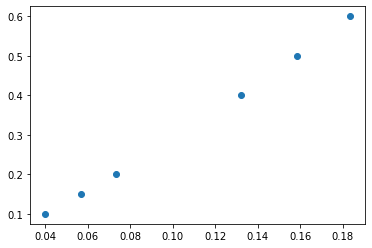
\includegraphics[width=\linewidth]{img/output.png}
        % \caption{$h/t - t$}
    \end{Figure}
    回归分析得到的结果:
    $$h/t = 4.944 t + 2.322$$

    由此测算:
    $$\widetilde g=9.889 m/s^2$$

    实验原理中第二种方法限于数据量较小、无法评估$t_0$的分布,结果不能达到精度要求。
    \subsection{结论}
    $$g=\widetilde g + \bar U_g =9.889 m/s^2\pm 0.0013 m/s^2, P=0.68$$
    
    实验数据:

    \bigskip
    \begin{tabular}{|c|c|c|c|c|}
        \hline \textbf{n} & \textbf{$h_1$} & \textbf{$h_2$} & \textbf{$t_1$} & \textbf{$t_2$} \\
        \hline $1$        & $30$           & $90$           & $243.4$         & $426.5$        \\
        \hline $2$        & $30$           & $90$           & $243.2$         & $426.3$        \\
        \hline $3$        & $30$           & $90$           & $243.5$         & $426.7$        \\
        \hline
        \hline $4$        & $30$           & $80$           & $243.6$         & $401.9$        \\
        \hline $5$        & $30$           & $80$           & $243.4$         & $401.7$        \\
        \hline $6$        & $30$           & $80$           & $243.3$         & $401.7$        \\
        \hline
        \hline $7$        & $30$           & $70$           & $243.5$         & $375.5$        \\
        \hline $8$        & $30$           & $70$           & $243.2$         & $375.2$        \\
        \hline $9$        & $30$           & $70$           & $243.6$         & $375.5$        \\
        \hline
        \hline $10$       & $20$           & $90$           & $197.1$         & $426.3$        \\
        \hline $11$       & $20$           & $90$           & $197.3$         & $426.4$        \\
        \hline $12$       & $20$           & $90$           & $197.4$         & $426.5$        \\
        \hline
        \hline $13$       & $20$           & $80$           & $197.3$         & $401.8$        \\
        \hline $14$       & $20$           & $80$           & $196.0$         & $400.5$        \\
        \hline $15$       & $20$           & $80$           & $197.8$         & $402.0$        \\
        \hline
        \hline $16$       & $20$           & $70$           & $197.4$         & $375.4$        \\
        \hline $17$       & $20$           & $70$           & $197.6$         & $375.5$        \\
        \hline $18$       & $20$           & $70$           & $197.6$         & $375.6$        \\
        \hline
        \hline $19$       & $30$           & $40$           & $241.6$         & $280.7$        \\
        \hline $20$       & $30$           & $40$           & $243.3$         & $282.5$        \\
        \hline $21$       & $30$           & $40$           & $243.5$         & $282.7$        \\
        \hline
        \hline $22$       & $30$           & $45$           & $243.6$         & $300.2$        \\
        \hline $23$       & $30$           & $45$           & $242.6$         & $299.4$        \\
        \hline $24$       & $30$           & $45$           & $242.9$         & $299.6$        \\
        \hline
        \hline $25$       & $30$           & $50$           & $243.8$         & $317.0$        \\
        \hline $26$       & $30$           & $50$           & $243.8$         & $316.9$        \\
        \hline $27$       & $30$           & $50$           & $242.7$         & $316.1$        \\
        \hline
        \hline $28$       & $35$           & $45$           & $263.7$         & $300.2$        \\
        \hline $29$       & $35$           & $45$           & $263.9$         & $300.4$        \\
        \hline $30$       & $35$           & $45$           & $264.5$         & $301.3$        \\
        \hline
        \hline $31$       & $40$           & $50$           & $281.0$         & $315.4$        \\
        \hline $32$       & $40$           & $50$           & $282.1$         & $316.4$        \\
        \hline $33$       & $40$           & $50$           & $281.4$         & $315.8$        \\
        \hline
        \hline $34$       & $45$           & $55$           & $299.3$         & $332.1$        \\
        \hline $35$       & $45$           & $55$           & $299.5$         & $332.3$        \\
        \hline $36$       & $45$           & $55$           & $299.7$         & $332.4$        \\
        \hline
    \end{tabular}
\end{multicols}
\end{document}